% Owner: TV1 (P5.1a) -- Reviewer: TV2
% Tables T1 and T3 are generated by `python -m experiments.report_tables`.
\subsection{Pruning on the $3\times 3$ Board, the Never-Lose Check, and the Effect of $c$}
\label{subsec:results_tv1}

\textbf{Alpha-beta versus Minimax (RQ1).} Table~\ref{tab:t1} counts the nodes visited when choosing the first move on the empty $3\times 3$ board with no depth limit. Every search returns the game value $0$ (a draw), and a unit test confirms that alpha-beta returns the Minimax value on $1\,000$ randomly sampled positions. Alpha-beta visits $96.7\%$ fewer nodes than Minimax with the natural (row-major) move order. The \emph{heuristic} order tries the cells that lie on the most winning lines first (center, then corners, then edges) and reduces the count by $98.7\%$, to $7\,275$ nodes. A random order, averaged over $20$ seeds, lies in between and varies by more than $1.5\times$ between seeds. As predicted by the analysis of Knuth and Moore~\cite{knuth1975analysis}, ordering good moves first is what makes the cut-offs happen early; even on this tiny tree it changes the cost by a factor of $2.5$.

\begin{table}[t]
\centering
\caption{T1: Nodes visited from the empty $3\times 3$ board (no depth limit)}
\label{tab:t1}
% Generated by experiments/report_tables.py -- do not edit by hand.
\begin{tabular}{lrr}
\toprule
Search & Nodes visited & Reduction \\
\midrule
Minimax & 549\,946 & -- \\
Alpha-beta, natural order & 18\,297 & 96.7\% \\
Alpha-beta, heuristic order & 7\,275 & 98.7\% \\
Alpha-beta, random order (20 seeds) & 14\,859 (11\,436--18\,125) & 97.3\% \\
\bottomrule
\end{tabular}

\end{table}

\textbf{When does MCTS stop losing? (RQ3).} Because MCTS is randomized, ``MCTS never loses'' is a statement about a fixed iteration budget and a fixed seed. We test it in two ways for $20$ seeds and both roles, with UCT constant $c = \sqrt{2}/2$ on the $[0,1]$ scale ($\sqrt{2}$ in our code), uniform random rollouts, and the most visited child as the final move. First, we walk the \emph{response tree}: MCTS plays its chosen move, the opponent tries \emph{every} legal reply, and we count the terminal positions in which MCTS loses. A seed passes only if no opponent strategy can beat it. Second, MCTS plays complete games against two perfect Minimax players (alpha-beta with natural order, and alpha-beta that breaks ties at random), in both roles.

\begin{table}[t]
\centering
\caption{T3: Never-lose check of MCTS on $3\times 3$ Tic-Tac-Toe ($20$ seeds, both roles; draws are out of $80$ games against perfect Minimax)}
\label{tab:t3}
% Generated by experiments/report_tables.py -- do not edit by hand.
\begin{tabular}{rrrr}
\toprule
Iterations & Seeds never losing & Losing lines & Draws vs.\ Minimax \\
\midrule
10 & 0/20 & 2\,024 & 36/80 \\
20 & 0/20 & 1\,437 & 34/80 \\
50 & 0/20 & 589 & 52/80 \\
100 & 0/20 & 367 & 61/80 \\
200 & 1/20 & 145 & 64/80 \\
500 & 2/20 & 42 & 75/80 \\
1\,000 & 15/20 & 16 & 80/80 \\
2\,000 & 20/20 & 0 & 80/80 \\
5\,000 & 20/20 & 0 & 80/80 \\
\bottomrule
\end{tabular}

\end{table}

Table~\ref{tab:t3} shows that losses fall steadily with the budget but disappear only late. The smallest budget in our grid at which all $20$ seeds survive the response tree and draw all $80$ games against Minimax, at that budget and every larger one, is $I^{*} = 2\,000$ iterations per move. The game-play test alone is too optimistic: at $1\,000$ iterations MCTS draws all $80$ games against Minimax, yet $5$ of the $20$ seeds still contain a losing line that a different opponent strategy would find. From $200$ iterations upward, every losing line occurs when MCTS plays second (as O). The typical trap is a corner opening by X answered with a move other than the center, after which X can create a double threat. This agrees with the regret analysis of Section~\ref{subsec:math_uct}: under uniform random rollouts the losing replies look almost as good as the correct reply, and separating two moves whose mean rewards differ by $\Delta$ needs on the order of $1/\Delta^2$ visits. Since $I^{*}$ is measured on a grid and over $20$ seeds, the true threshold lies between $1\,000$ and $2\,000$ iterations for this configuration.

\textbf{Interaction of $c$ and the budget (RQ4).} Figures~\ref{fig:f1} and~\ref{fig:f2} show the win rate of MCTS with uniform random rollouts against a random player, for $c \in \{0.5, 1.0, 1.4, 2.0\}$ on the $[0, 1]$ scale and $100$ to $5\,000$ iterations, with $200$ games per point, the first move alternated, and $95\%$ Wilson intervals. On $3\times 3$ Tic-Tac-Toe the curves are flat: MCTS wins between $90.5\%$ and $98\%$ of the games and draws the rest, it loses at most $6$ of $200$ games and only at $100$ iterations, and the differences between values of $c$ are within the confidence intervals. On $9\times 9$ Gomoku the constant matters when the budget is small. At $100$ iterations the win rate decreases monotonically with $c$, from $96.5\%$ at $c = 0.5$ to $88.5\%$ at $c = 2.0$ (two-proportion $z = 3.04$, $p = 0.002$). From $500$ iterations upward every configuration wins at least $99\%$ of the games. With few iterations and several dozen candidate moves at the root, a large $c$ spreads the visits almost uniformly and leaves too few for the promising moves; a larger budget hides this cost. A random opponent saturates quickly, so finer differences between configurations are measured against stronger opponents in Sections~\ref{subsec:results_tv2} and~\ref{subsec:results_tv3}.

\begin{figure}[t]
\centering
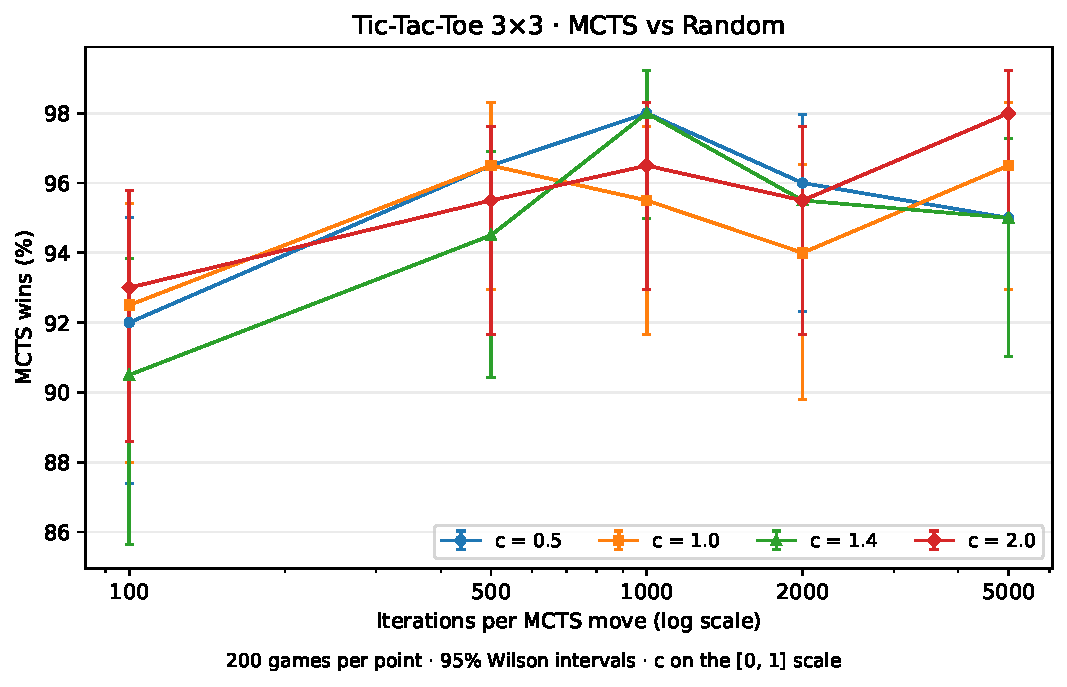
\includegraphics[width=\columnwidth]{figures/F1.pdf}
\caption{F1: Win rate of MCTS against a random player on $3\times 3$ Tic-Tac-Toe versus iterations, one curve per value of $c$ ($[0,1]$ scale, $200$ games per point, $95\%$ Wilson intervals).}
\label{fig:f1}
\end{figure}

\begin{figure}[t]
\centering
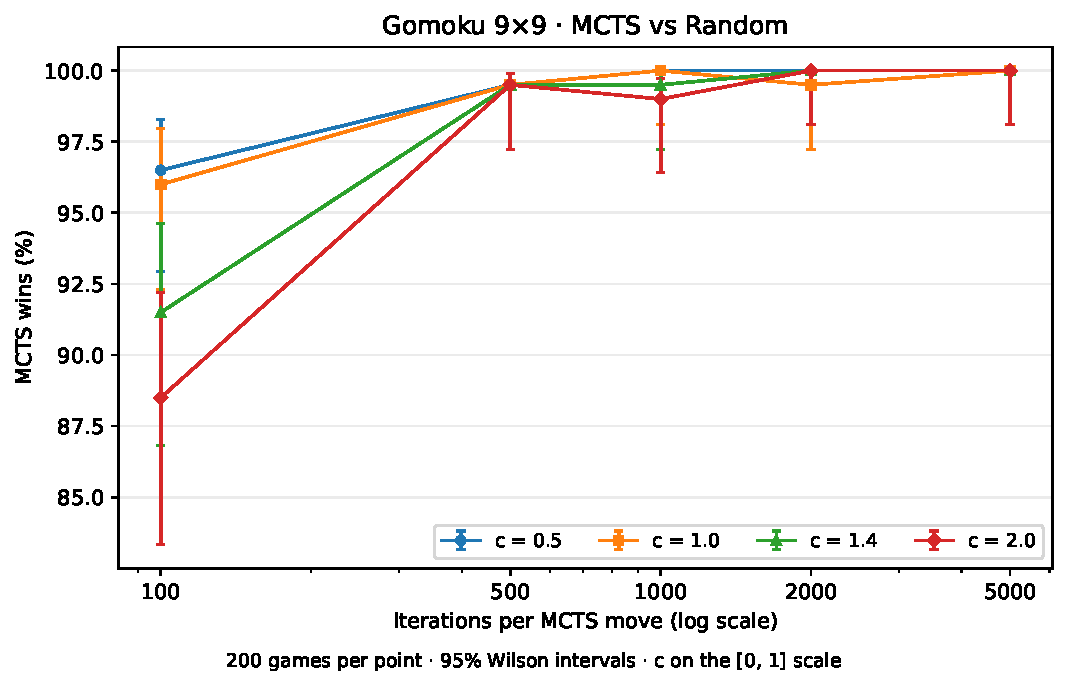
\includegraphics[width=\columnwidth]{figures/F2.pdf}
\caption{F2: Win rate of MCTS against a random player on $9\times 9$ Gomoku versus iterations, one curve per value of $c$ ($[0,1]$ scale, $200$ games per point, $95\%$ Wilson intervals).}
\label{fig:f2}
\end{figure}
